\begin{itemize}
    \item
        Weshalb wurde das benutzte mathematische Modell gew\"ahlt?
    \item
        Weshalb wird ein Schaltregler benutzt?
    \item
        Weshalb wurde ein eigenes PCB entwickelt statt ein Steckbrett verwendet?
    \item
        Wie soll unser Ger\"at bedient werden k\"onnen?
\end{itemize}

Underpinning  our  device  is  a  microcontroller which  has  as  its  primary
responsibilities the  handling of IO tasks  (such as user interaction  and the
display) and  controlling the step-down converter. Power  delivery is realised
with a prebuilt DC power supply unit as per the requirements.

With  an  eye towards  potential  serial  production,  a proprietary  PCB  was
developed.  This allows tight control  over impedances in the lines connecting
critical  components and  brings the  behavior  of the  prototype device  much
closer  to  a mass  produced  version  than  a breadboard  solution  could. It
should  also  be  pointed  out  that  trace  routing,  lengths  and  component
placement are crucial,  as is discussed in  section \ref{sec:verification} (p.
\pageref{sec:verification}ff), \emph{Verification}.

Interaction with  our device can  be done both  via physical interface  on the
device itself,  which is comprised  of a display  and a push-twist  button, as
well as  on a PC  connected by USB  using our software  \emph{Smooth} (section
\ref{subsec:frontend}, p. \pageref{subsec:frontend}ff).


% **************************************************************************** %
\subsection{Concept of Regulation Circuit}
% **************************************************************************** %

\begin{minipage}{0.5\textwidth}
    \center
    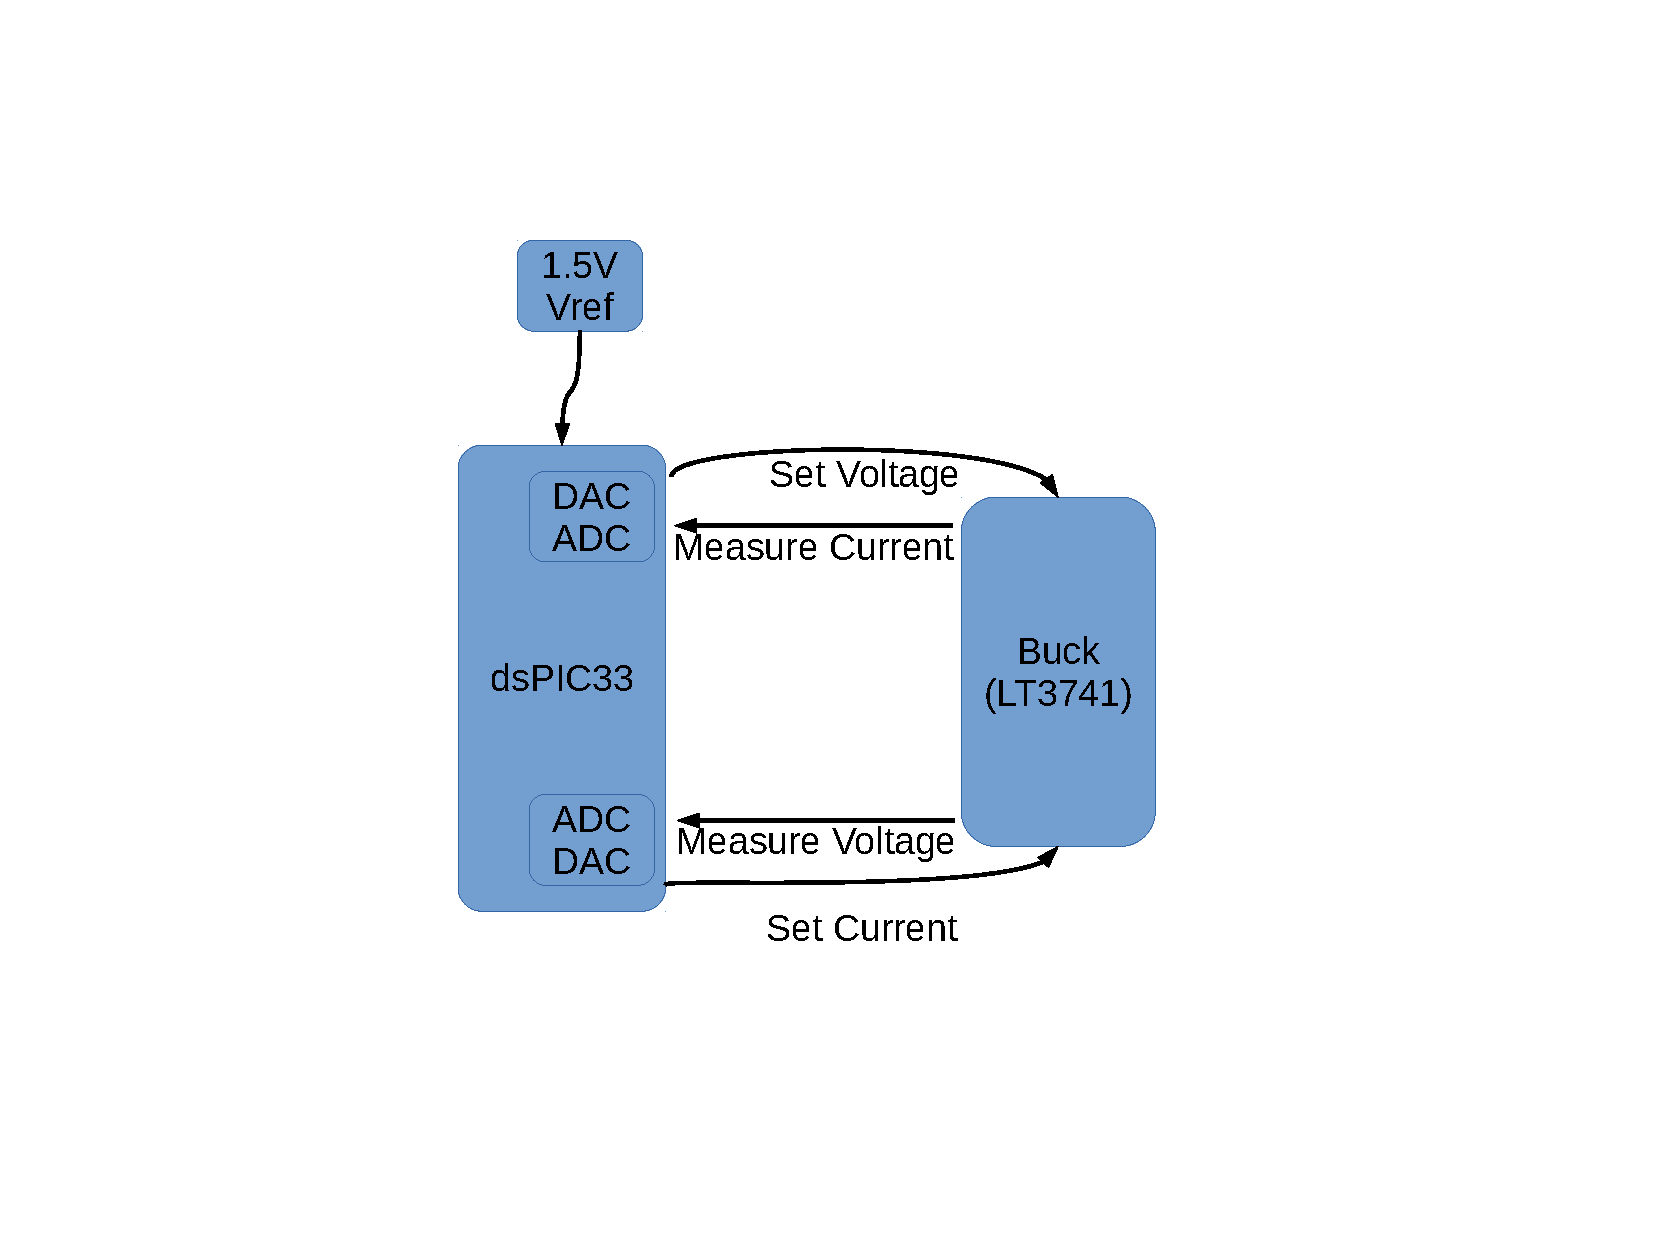
\includegraphics[width=\textwidth,trim=140 140 120 100,clip]{images/block-diag-control.pdf}
    \captionof{figure}{Block diagram of control circuit}
    \label{fig:diag:block}
\end{minipage}
\begin{minipage}{0.5\textwidth}
    \center
    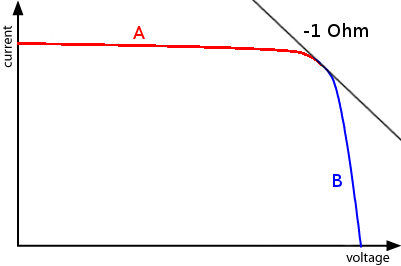
\includegraphics[width=\textwidth]{images/vi-curve.png}
    \captionof{figure}{VI-Curve with \SI{-45}{\degree} slope indicated}
    \label{fig:circuit:buck:uset}
\end{minipage}


\subsection{Goals of the model}
Our aim is to have a simple model, as usability is more important than accuracy. In other words, our model should have a small set of parameters, which can be easily determined by the user. Further it must respect solar irradiation, as we want to model how clouded skies or a partially covered module affects its output.

\subsection{Model for one solar cell}
As Basis for our model serves the single diode model of the ideal PV cell \todo{comprehensive appr}. The I-V characteristic of this circuit is
\begin{equation}
 I = I_{pv,cell} - I_{o,cell} \left[ \exp \left( \frac{qV}{akT} \right) - 1 \right]
 \end{equation}
